\documentclass{beamer}
\usepackage[utf8]{inputenc}
\usepackage{hyperref}

\usepackage{graphicx}
\usepackage{caption}
\usepackage{subcaption}
\usepackage{amsmath}
\usepackage{listings}
\usepackage{color}
\definecolor{mygreen}{RGB}{28,172,0} % color values Red, Green, Blue
\definecolor{mylilas}{RGB}{170,55,241}
\lstset{language=Matlab,%
    basicstyle=\footnotesize,
    breaklines=true,%
    morekeywords={matlab2tikz},
    keywordstyle=\color{blue},%
    morekeywords=[2]{1}, keywordstyle=[2]{\color{black}},
    identifierstyle=\color{black},%
    stringstyle=\color{mylilas},
    commentstyle=\color{mygreen},%
    showstringspaces=false,%without this there will be a symbol in the places where there is a space
    numbers=left,%
    numberstyle={\tiny \color{black}},% size of the numbers
    numbersep=9pt, % this defines how far the numbers are from the text
    emph=[1]{for,end,break},emphstyle=[1]\color{red}, %some words to emphasise
    %emph=[2]{word1,word2}, emphstyle=[2]{style},
}
\title[Real-Time Spectrum Analyser~~~~~~~~~~~~~~~~~~~~~~~~~~~~~~~~~~\insertframenumber/\inserttotalframenumber]{Implementation of a Real-Time Spectrum Analyzer Synthesized on FPGA}
\author[David Lavoie-Boutin]{David Lavoie-Boutin, 260583602}
\date{\today}

\usetheme{Copenhagen}
\usecolortheme{beaver}

\begin{document}

\frame{\titlepage}

\begin{frame}
\frametitle{Table of Contents}
\tableofcontents
\end{frame}

\section{Motivation}

\begin{frame}\frametitle{FFT is useful }

  \begin{exampleblock}{}
    {\large ``The most important numerical algorithm of our lifetime''}
    \vskip5mm
    \hspace*\fill{\small--- Gilbert Strang}
  \end{exampleblock}
\end{frame}

\begin{frame}
  \frametitle{Steps}
  \begin{itemize}
    \item Matlab Implementation
    \item Code Generation
    \item Display Module
    \item Full Integration
  \end{itemize}
\end{frame}

\section{Matlab}

\begin{frame}
  \frametitle{Cooley–Tukey Algorithm}
  \lstinputlisting[language=Matlab, firstline=3, lastline=14, caption=Recursive FFT implementation]{../myFFT.m}
\end{frame}

\begin{frame}
  \lstinputlisting[language=Matlab, caption=Iterative FFT implementation, lastline=5]{../fft_it.m}
\end{frame}


\begin{frame}
  \frametitle{Simulink schematic}
  \begin{figure}[!htb]
    \centering
    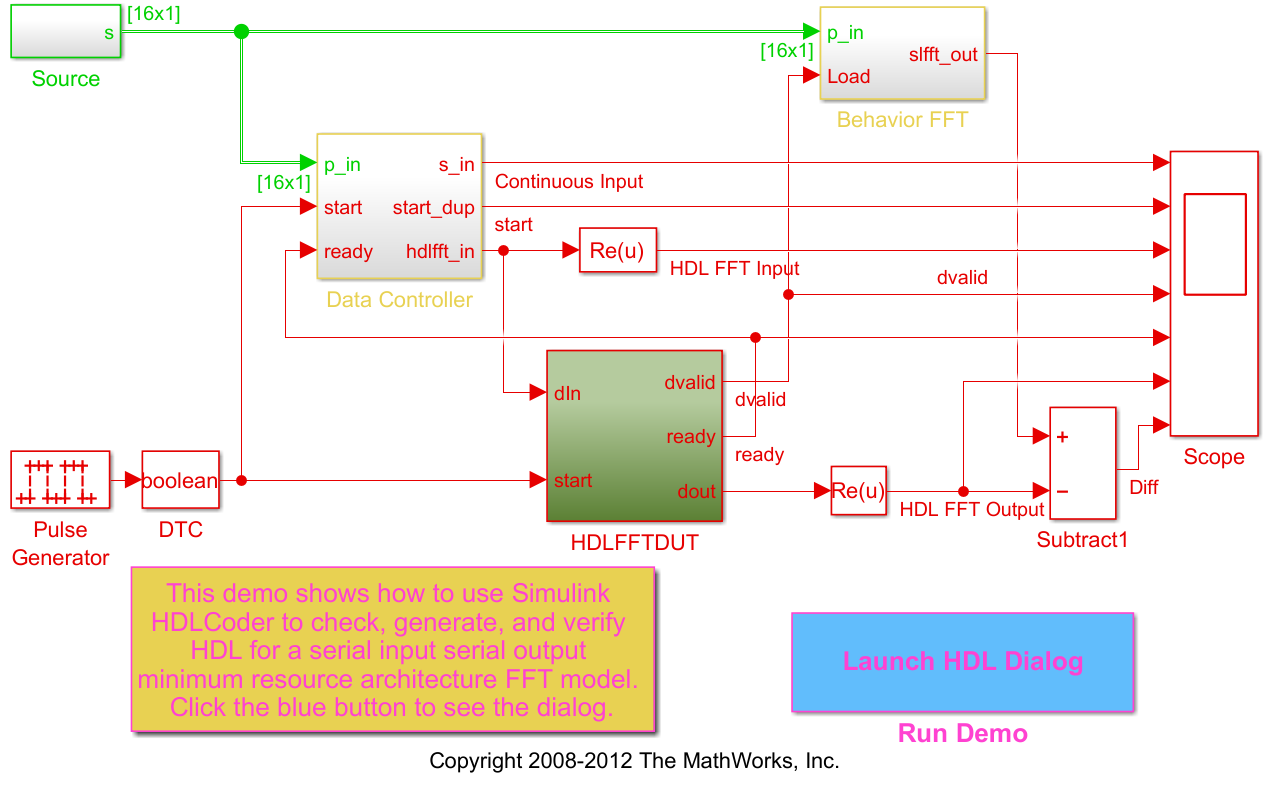
\includegraphics[width=0.8\textwidth]{sim2.PNG}
    \caption{Simulink schematic of a HDL optimized FFT}
    \label{fig:simulink}
  \end{figure}
\end{frame}

\section{Display on the FPGA}
\begin{frame}\frametitle{Display module using switches}
  \begin{figure}[!htb]
    \centering
    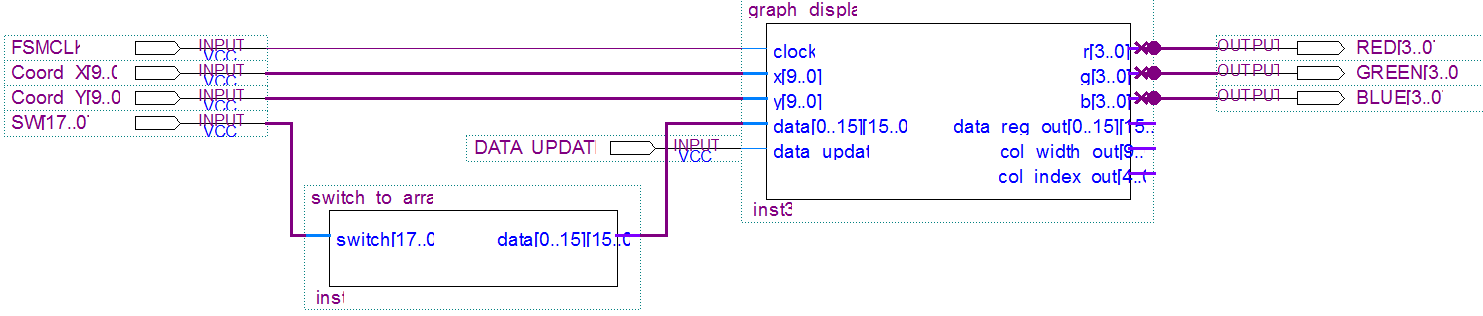
\includegraphics[width=0.8\textwidth]{switch_circuit.PNG}
  \end{figure}
\end{frame}


\begin{frame}\frametitle{Package Definitions}
\lstinputlisting[language=VHDL, firstline=5, lastline=10]{../VideoLab/graph_display.vhd}
\end{frame}

\begin{frame}\frametitle{Modular Bar Chart}
\lstinputlisting[language=VHDL, firstline=47, lastline=49]{../VideoLab/graph_display.vhd}
\end{frame}

\begin{frame}\frametitle{Array Input}
\lstinputlisting[language=VHDL]{array_ex.vhd}
\end{frame}

\begin{frame}\frametitle{Switch to Test}
\lstinputlisting[language=VHDL, firstline=7, lastline=12]{../VideoLab/switch_to_array.vhd}
\begin{figure}[!htb]
  \centering
  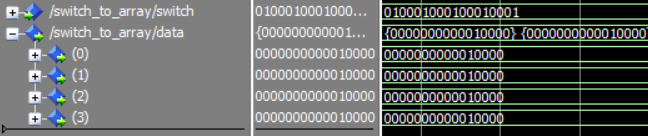
\includegraphics[width=0.8\textwidth]{switch_sim.PNG}
  \caption{Modelsim simulation of the switch to array module}
  \label{fig:switch_sim}
\end{figure}
\end{frame}

\section{FFT on FPGA}

\begin{frame}\frametitle{Audio processing pipeline}
\begin{figure}[!htb]
  \centering
  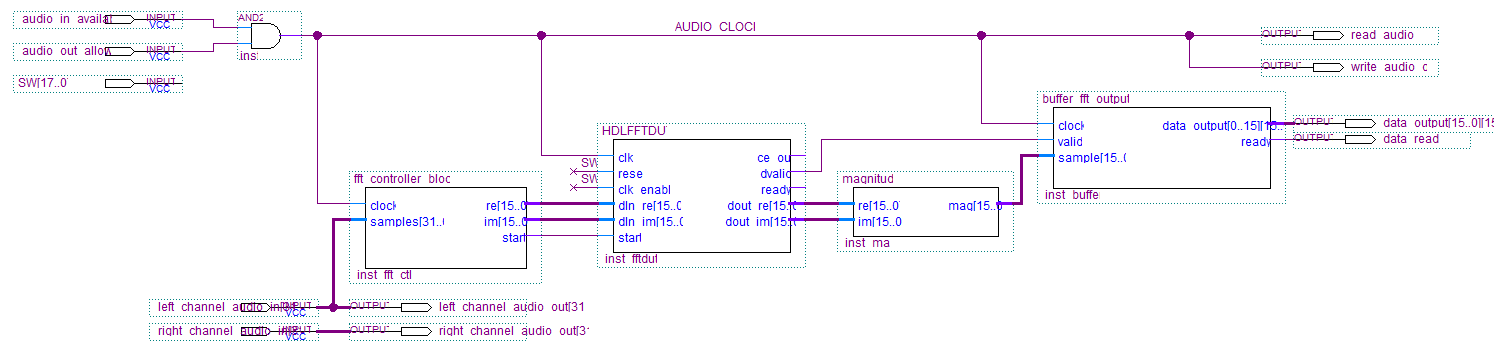
\includegraphics[width=\textwidth]{full_filter.PNG}
  \caption{FFT integration in the audio processing unit}
  \label{fig:block_filter}
\end{figure}
\end{frame}

\begin{frame}\frametitle{FFT Controller}
\lstinputlisting[language=VHDL, firstline=18, lastline=34]{../VideoLab/fft_controller_block.vhd}
\end{frame}

\begin{frame}\frametitle{Magnitude of complex number}
\lstinputlisting[language=VHDL, firstline=5, lastline=8, caption=Square-Root function]{../VideoLab/sqrt.vhd}
\lstinputlisting[language=VHDL, firstline=18, lastline=20, caption=Magnitude module]{../VideoLab/magnitude.vhd}
Non-Restoring Square Root Algorithm
\end{frame}

\begin{frame}\frametitle{Data buffer}
\lstinputlisting[language=VHDL, firstline=7, caption=Buffer module for the FFT output, lastline=16]{../VideoLab/buffer_fft_output.vhd}
\end{frame}

\begin{frame}\frametitle{Data buffer}

\begin{figure}[!htb]
  \centering
  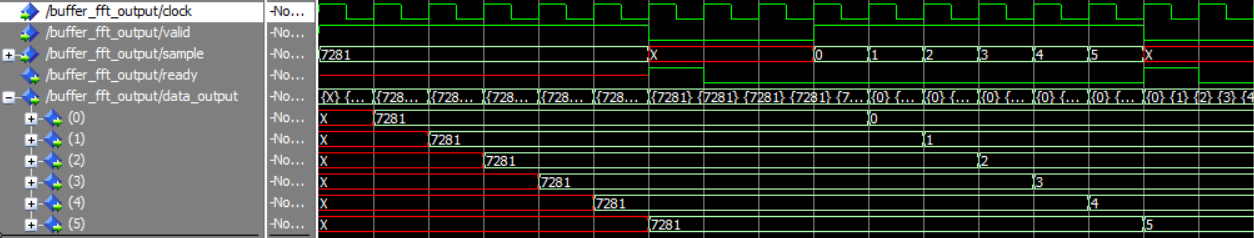
\includegraphics[width=\textwidth]{buffer_sim.PNG}
  \caption{Simulation results for the buffer module}
  \label{fig:buff_sim}
\end{figure}
\end{frame}

\begin{frame}\frametitle{Audio processing pipeline}
\begin{figure}[!htb]
  \centering
  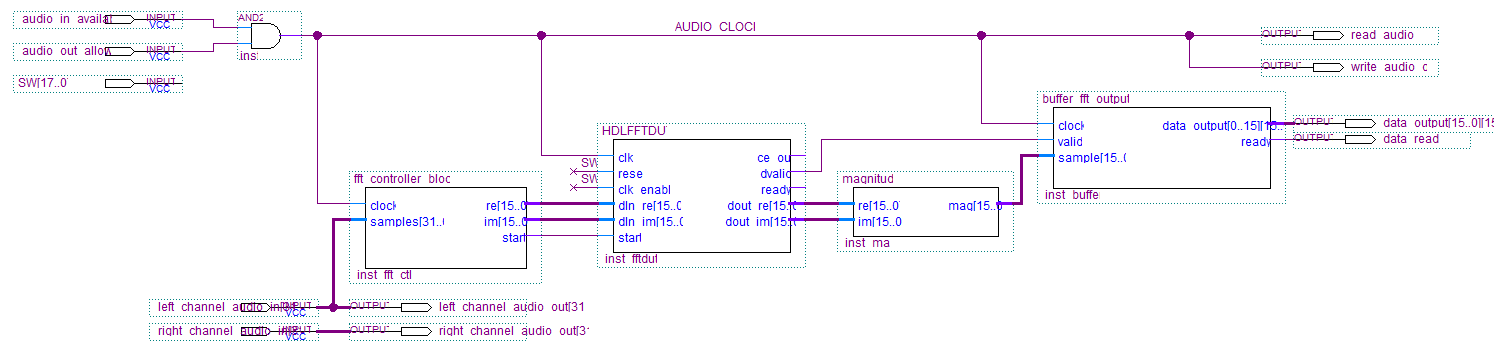
\includegraphics[width=\textwidth]{full_filter.PNG}
\end{figure}
\end{frame}

\begin{frame}\frametitle{Full Design}
\begin{figure}[!htb]
  \centering
  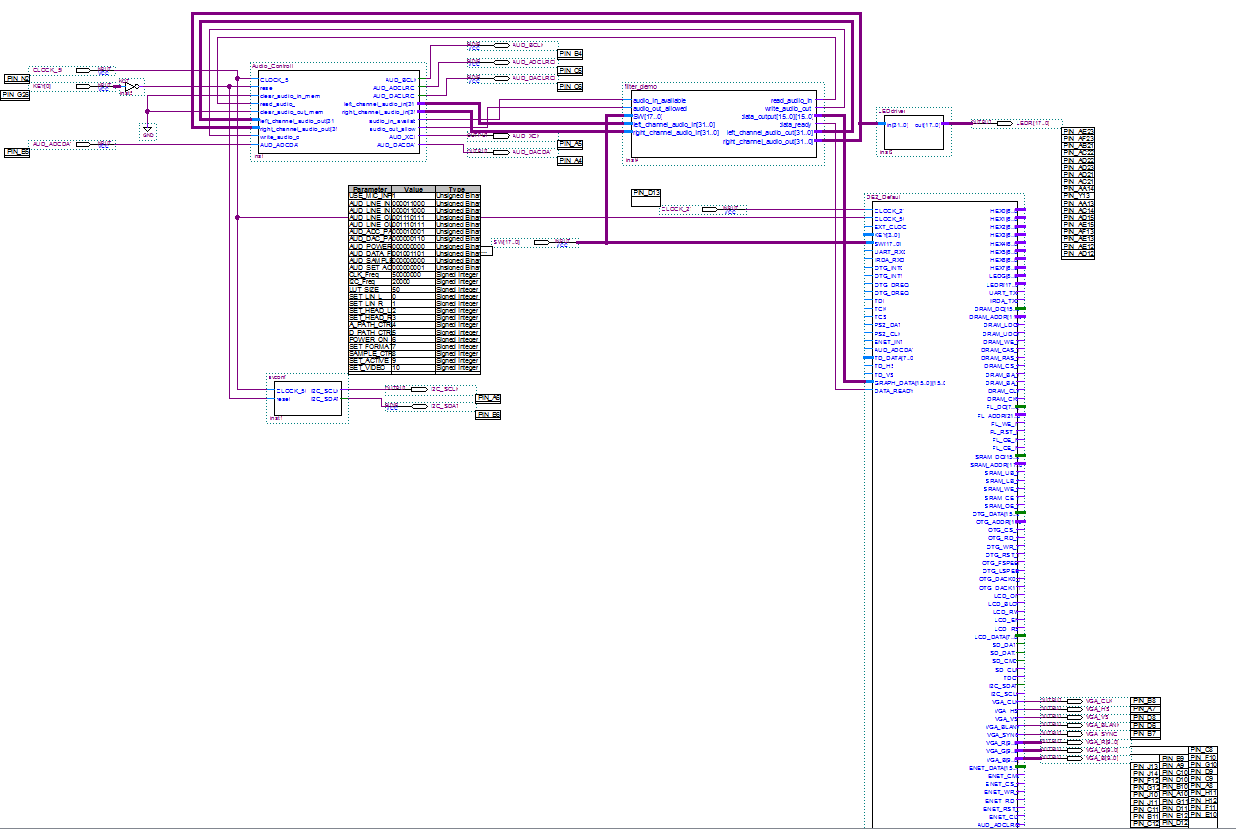
\includegraphics[width=\textwidth]{top_level.PNG}
\end{figure}
\end{frame}


\end{document}